\documentclass[a4paper,12pt]{article} 
%%%%%%%%%%%%%%%%%%%%%%%%%%%%%%%% CONSTANTES %%%%%%%%%%%%%%%%%%%%%%%%%%%%%%%%%%%
\newcommand{\numero}{9}                                    %Numéro de la série -1

\usepackage[french]{babel}
\usepackage[utf8]{inputenc}
\usepackage{answers}

\usepackage{hyperref}
\usepackage{multicol}

\usepackage[table,xcdraw]{xcolor}
\usepackage{listings}
\definecolor{ForestGreen}{RGB}{34,139,34}


\usepackage{enumitem}

\AtBeginDocument{\def\labelitemi{$\bullet$}}


\newcommand{\py}{\lstinline{Python} }


\definecolor{backcolour}{rgb}{0.95,0.95,0.92}

\lstset{%
	language         = Python,
	backgroundcolor  = \color{backcolour},
	basicstyle       = \ttfamily, % \upshape\ttfamily,
	keywordstyle     = \bfseries\color{blue}, %\bfseries,
	stringstyle      = \color{magenta},
	commentstyle     = \color{ForestGreen},
	alsoletter = > ,
	morekeywords = {>>>,as,assert,False,None, nonlocal,True, with,yield , <<, >>, :},
	showstringspaces = false,
	numbers=left,
	stepnumber=1,
	literate={à}{{\`{a}}}1 {é}{{\'e}}1 {è}{{\`{e}}}1 {ê}{{\^{e}}}1 {Ê}{{\^{E}}}1 {î}{{\^i}}1 {ô}{{\^{o}}}1 {ç}{{\c{c}}}1 {Ç}{{\c{C}}}1
}

\newcommand{\itemb}[1]{\item \textbf{#1}}

\usepackage{fancyhdr}  %package pour en-tetes et pied de pages
\usepackage{sectsty} % Permet de faire des modifications de police dans diverses sections des "headings" (cf. modif presentation de la page)
\pagestyle{fancy}       %Style pour en-tetes et pieds de pages
\fancyhead[CO,CE]{\sc Série 1\hspace{0.5mm}}
\fancyhead[RO,LE]{Collège Sismondi}  % LaTeX/TEX define \strut to be an invisible box of width zero that extends just enough above and below the baseline. Cela permet d'augementer légèrement la taille en bas de la box de manière à ce qu'elle soit collée à la ligne.
\fancyhead[LO,RE]{\small\ \textsl{1\textsuperscript{ère} année - DO Informatique}}
\fancyfoot[RO,LE]{2021 - 2022}
\fancyfoot[LO,RE]{\small }
\fancyfoot[CO,CE]{\thepage}

\fancyhfoffset[l]{1.2cm} % le "l" en paramètre permet d'indiquer qu'on ne veut modifier que la marge à gauche.
\renewcommand{\headrule}{{%
		\hrule \headwidth \headrulewidth \vskip-\headrulewidth}}
\renewcommand\footrulewidth{\headrulewidth}
\renewcommand{\footrule}{{%
		\vskip-\footruleskip\vskip-\footrulewidth
		\hrule \headwidth \footrulewidth\vskip\footruleskip}}

\usepackage{tikz}
%-------------------------------------------------------------------------------
%---- Eclairage : en encadré sur fond jaune avec symbôle "ampoule" à gauche ----
%-------------------------------------------------------------------------------
\definecolor{coleclairage}{RGB}{255 , 221 , 156}
\definecolor{contoureclairage}{RGB}{255 , 192 , 0}
\newenvironment{eclairage}
{
	\begin{center}%
		\begin{tikzpicture}%
			\node[rectangle, draw=contoureclairage, top color=coleclairage!50, bottom color=coleclairage!140, rounded corners=5pt, inner xsep=5pt, inner ysep=6pt, outer ysep=10pt]\bgroup                     
			\begin{minipage}{0.98\linewidth}
				\begin{minipage}{0.08\linewidth}\centerline{
\includegraphics[scale=1]{Symbole_eclairage.png}}\end{minipage}
				\begin{minipage}{0.89\linewidth}\itshape\footnotesize
				}
				{                		
				\end{minipage}
			\end{minipage}\egroup;%
		\end{tikzpicture}%
	\end{center}%
}

%-------------------------------------------------------------------------------
%---- apprendre : en encadré sur fond jaune avec symbôle "ampoule" à gauche ----
%-------------------------------------------------------------------------------
\definecolor{colapprendre}{RGB}{50,205,50}
\definecolor{contourapprendre}{RGB}{34,139,34}
\newenvironment{apprendre}
{
	\begin{center}%
		\begin{tikzpicture}%
			\node[rectangle, draw=contourapprendre, top color=colapprendre!10, bottom color=colapprendre!50, rounded corners=5pt, inner xsep=5pt, inner ysep=6pt, outer ysep=10pt]\bgroup                     
			\begin{minipage}{0.98\linewidth}
				\begin{minipage}{0.08\linewidth}\centerline{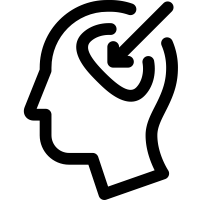
\includegraphics[width=30px]{Symbole_learn.png}}\end{minipage}
				\begin{minipage}{0.89\linewidth}\itshape\footnotesize
				}
				{                		
				\end{minipage}
			\end{minipage}\egroup;%
		\end{tikzpicture}%
	\end{center}%
}

\definecolor{colimportant}{RGB}{247 , 189 , 164}
\definecolor{contourimportant}{RGB}{237 , 125 , 49}
\newenvironment{important}
{
	\begin{center}%
		\begin{tikzpicture}%
			\node[rectangle, draw=contourimportant, top color=colimportant!50, bottom color=colimportant!140, rounded corners=5pt, inner xsep=5pt, inner ysep=6pt, outer ysep=10pt]\bgroup                     
			\begin{minipage}{0.08\linewidth}\centerline{
\includegraphics[scale=0.8]{Symbole_attention.png}}\end{minipage}
			\begin{minipage}{0.89\linewidth}
			}
			{                		
			\end{minipage}\egroup;
		\end{tikzpicture}%
	\end{center}%
}

%-----------------------------------------------------------------
%---- Modification présentation de la page: marges de la page ----
%-----------------------------------------------------------------
%\addtolength{\hoffset}{-1in}              % 1
%\addtolength{\voffset}{-1in}              % 2
\addtolength{\oddsidemargin}{-0.1 in} % 3
\addtolength{\evensidemargin}{-1in} % 3
\addtolength{\topmargin}{-1in}       % 4
\addtolength{\headheight}{6pt}       % 5
%\addtolength{\headsep}{-0.2cm}           % 6
\setlength{\textheight}{26cm}    % 7
\setlength{\textwidth}{16.5cm}      % 8
\addtolength{\marginparsep}{0pt}      % 9
\setlength{\marginparwidth}{0pt}   % 10
\addtolength{\footskip}{-1mm}           %11

\setlength{\parindent}{0em}% pas d'indentation


% Customiser le nom des sections
\usepackage{titlesec}
\titleformat{\section}[hang]{\Large \bfseries}{Série \thesection:\ }{0pt}{}

\renewcommand{\familydefault}{\sfdefault} % pour avoir des polices san serif

\newtheorem{Exc}{Exercice}
\Newassociation{correction}{Soln}{mycor}
\renewcommand{\Solnlabel}[1]{\bfseries Ex #1 }
\def\exo#1{%
	\futurelet\testchar\MaybeOptArgmyexoo}
\def\MaybeOptArgmyexoo{
	\ifx[\testchar \let\next\OptArgmyexoo
	\else \let\next\NoOptArgmyexoo \fi \next}
\def\OptArgmyexoo[#1]{%
	\begin{Exc}[#1]\normalfont}
	\def\NoOptArgmyexoo{%
		\begin{Exc}\normalfont}
		\newcommand{\finexo}{\end{Exc} \vspace{3mm}}
	\newcommand{\flag}[1]{}
	\newcommand{\entete}[1]

\newcommand{\getexocompteur}{{\the\numexpr \arabic{Exc}  \relax}}	
	
\newcommand{\eexo}{\vspace{5mm}} % espace pour séparer les exercices

\begin{document}
%		\title{\vspace{-3cm}Série 1}
%		\date{\vspace{-2cm}}
%		\maketitle

\fancyhead[CO,CE]{\sc Série \arabic{section} \hspace{0.5mm}}

\setcounter{section}{\numero}
\section{Les Boucles}				
\Opensolutionfile{mycor}[cor_01]

\exo{}  ~\\ 
Écrire un programme qui détermine si une année entrée par l’utilisateur est bissextile ou non.
Pour savoir si une année A est bissextile il faut qu’une des conditions suivantes soit vérifiée :
\begin{itemize}
	\item si l'année est divisible par 4 et non divisible par 100 ;
	\item si l'année est divisible par 400.
\end{itemize}
Vérifier que 2000, 2024, 2028 et 2032 sont des années bissextiles mais que 2021, 2022 et 1900 ne sont pas des années  bissextiles.
\begin{correction}
	~\\ 
	\textbf{Première version :}
	\lstinputlisting[numbers=none]{codes/ex0_corrige.py}
	
	\textbf{Deuxième version :}	
	\lstinputlisting[numbers=none]{codes/ex0_corrigeb.py}	
	
\end{correction}
\finexo

\exo{}  ~\\ 
Soit le programme suivant:
\lstinputlisting[numbers=none]{codes/ex1.py}
\begin{enumerate}
	\item Qu’affichera le programme en sortie? Vérifier votre réponse en exécutant le programme sur l'exécuteur pas à pas \url{http://pythontutor.com/visualize.html#mode=edit}.
	\item Écrire et tester un programme qui affiche tous les entiers pairs compris entre 18 et 45.\\
	\textit{Pour tester qu'un nombre \lstinline{n} est pair on peut caluler le reste de la division par 2 : }\lstinline!n % 2 == 0!
	\item Écrire et tester un programme qui affiche tous les entiers impairs compris entre 50 et 150.
	\textit{Pour tester qu'un nombre \lstinline{n} est pair on peut caluler le reste de la division par 2 : }\lstinline!n % 2 == 1!
\end{enumerate}
\begin{correction}
	~\\ 
	\textbf{2.}\lstinputlisting[numbers=none]{codes/ex1_corrige_2.py}
	\textbf{3.} \lstinputlisting[numbers=none]{codes/ex1_corrige_3.py}
\end{correction}
\finexo

\exo{}  ~\\ 
Écrire et tester un programme permettant de calculer la somme des entiers naturels pairs inférieurs ou égaux à 1000
\begin{correction}
	~\\ 
	\lstinputlisting[numbers=none]{codes/ex3_corrige.py}
\end{correction}
\finexo

\exo{}  ~\\ 
On place un capital de 500CHF sur un compte rémunéré à 3% par an.
Le programme ci-dessous a pour but de calculer le nombre d'années au bout desquelles le capital sera doublé. 
\lstinputlisting[numbers=none]{codes/ex4.py}
Le problème est que le programme contient une erreur !
\begin{enumerate}
	\item Corriger le programme afin qu’il atteigne le but espéré, puis le tester.
	\item Modifier le programme précédent de telle sorte que le capital et le taux de rémunération soient saisis en entrée. Le tester dans un nouveau contexte à décrire (avec de nouvelles valeurs).
\end{enumerate}
\begin{correction}
	~\\ 
	\begin{enumerate}
		\item 	\lstinputlisting[numbers=none]{codes/ex4_corrige_1.py}
		\item 	\lstinputlisting[numbers=none]{codes/ex4_corrige_2.py}
	\end{enumerate}
	
	\lstinputlisting[numbers=none]{codes/ex4_corrige_1.py}
\end{correction}

\finexo

\exo{}  ~\\ 
Le jeu des allumettes : ce jeu se joue à deux joueurs. Au départ 30 allumettes sont disposées. Puis, à tour de rôle, chaque joueur enlève au maximum 3 allumettes. Le joueur qui prend la dernière allumette a perdu ! Exemple d’affichage: 
\begin{correction}
	~\\ 
	\lstinputlisting[numbers=none]{codes/ex3_corrige.py}
\end{correction}
\finexo

\exo{}[Apprendre en  autonomie avec france IOI]  ~\\ 
Allez sur le site de france IOI sur \url{http://www.france-ioi.org/}, puis valider la séquence 8 "\textit{Répétitions conditionnées}".
\finexo

\exo{}[facultatif, pour les matheux !]  ~\\ 
Une tortue s'élance sur une piste de 10 mètres de long. Le jour, elle parcourt 1 mètre, la nuit, elle se repose.
\vspace{3mm}
Seulement, voilà, la piste, en caoutchouc, s'étire toutes les nuits de 10 mètres. Ainsi, au deuxième matin, la tortue se retrouve à deux mètres du début de la piste, mais à 18 mètres de son extrémité. Lorsqu'elle s'endort le soir, il lui reste encore 17 mètres à parcourir. 
\vspace{3mm}
Et lorsqu'elle se réveille le matin suivant, la piste a 30 mètres de long, dont plus de 25 mètres sont devant elle!
\begin{enumerate}
	\item La tortue arrivera-t-elle au bout de la piste?
	\item Si oui, en combien de temps?
	\item Rédiger un script qui détermine le nombre de jours.
\end{enumerate}

\textit{Indication : calculer la fraction de la piste que la tortue parcours chaque jour.}


\finexo

\cleardoublepage


% Solution		
		\newpage
		\setcounter{page}{1}
		\setcounter{section}{\numero}
		\Closesolutionfile{mycor}
		\titleformat{\section}[hang]{\Large \bfseries}{Corrigé Série \thesection:\ }{0pt}{}
		

		\fancyhead[CO,CE]{\sc Corrigé Série \arabic{section} \hspace{0.5mm}}
		\section{}
		\Readsolutionfile{mycor}
	\end{document}